\documentclass{article}

\usepackage{fancyhdr}
\usepackage{extramarks}
\usepackage{amsmath}
\usepackage{amsthm}
\usepackage{amsfonts}
\usepackage{tikz}
\usepackage[plain]{algorithm}
\usepackage{algpseudocode}
\usepackage{float}

\usetikzlibrary{automata,positioning}

%
% Basic Document Settings
%

\topmargin=-0.45in
\evensidemargin=0in
\oddsidemargin=0in
\textwidth=6.5in
\textheight=9.0in
\headsep=0.25in

\linespread{1.1}

\pagestyle{fancy}
\lhead{\hmwkAuthorName}
\chead{\hmwkClass\: \hmwkTitle}
\rhead{\firstxmark}
\lfoot{\lastxmark}
\cfoot{\thepage}

\renewcommand\headrulewidth{0.4pt}
\renewcommand\footrulewidth{0.4pt}

\setlength\parindent{0pt}

%
% Create Problem Sections
%

\newcommand{\enterProblemHeader}[1]{
    \nobreak\extramarks{}{Problem \arabic{#1} continued on next page\ldots}\nobreak{}
    \nobreak\extramarks{Problem \arabic{#1} (continued)}{Problem \arabic{#1} continued on next page\ldots}\nobreak{}
}

\newcommand{\exitProblemHeader}[1]{
    \nobreak\extramarks{Problem \arabic{#1} (continued)}{Problem \arabic{#1} continued on next page\ldots}\nobreak{}
    \stepcounter{#1}
    \nobreak\extramarks{Problem \arabic{#1}}{}\nobreak{}
}

\setcounter{secnumdepth}{0}
\newcounter{partCounter}
\newcounter{homeworkProblemCounter}
\setcounter{homeworkProblemCounter}{1}
\nobreak\extramarks{Problem \arabic{homeworkProblemCounter}}{}\nobreak{}

%
% Homework Problem Environment
%
% This environment takes an optional argument. When given, it will adjust the
% problem counter. This is useful for when the problems given for your
% assignment aren't sequential. See the last 3 problems of this template for an
% example.
%
\newenvironment{homeworkProblem}[1][-1]{
    \ifnum#1>0
        \setcounter{homeworkProblemCounter}{#1}
    \fi
    \section{Problem \arabic{homeworkProblemCounter}}
    \setcounter{partCounter}{1}
    \enterProblemHeader{homeworkProblemCounter}
}{
    \exitProblemHeader{homeworkProblemCounter}
}

%
% Homework Details
%   - Title
%   - Due date
%   - Class
%   - Section/Time
%   - Instructor
%   - Author
%

\newcommand{\hmwkTitle}{Lab\ \#1}
\newcommand{\hmwkDueDate}{February 12, 2014}
\newcommand{\hmwkClass}{EE 133}
\newcommand{\hmwkClassTime}{Section A}
\newcommand{\hmwkClassInstructor}{Professor Isaac Newton}
\newcommand{\hmwkAuthorName}{\textbf{John Kustin}}

%
% Title Page
%

\title{
    \vspace{2in}
    \textmd{\textbf{\hmwkClass:\ \hmwkTitle}}\\
    \normalsize\vspace{0.1in}\small{Due\ on\ \hmwkDueDate\ at 5pm}\\
    % \vspace{0.1in}\large{\textit{\hmwkClassInstructor\ \hmwkClassTime}}
    \vspace{3in}
}

\author{\hmwkAuthorName}
\date{}

\renewcommand{\part}[1]{\textbf{\large Part \Alph{partCounter}}\stepcounter{partCounter}\\}

%
% Various Helper Commands
%

% Useful for algorithms
\newcommand{\alg}[1]{\textsc{\bfseries \footnotesize #1}}

% For derivatives
\newcommand{\deriv}[1]{\frac{\mathrm{d}}{\mathrm{d}x} (#1)}

% For partial derivatives
\newcommand{\pderiv}[2]{\frac{\partial}{\partial #1} (#2)}

% Integral dx
\newcommand{\dx}{\mathrm{d}x}

% Alias for the Solution section header
\newcommand{\solution}{\textbf{\large Solution}}

% Probability commands: Expectation, Variance, Covariance, Bias
\newcommand{\E}{\mathrm{E}}
\newcommand{\Var}{\mathrm{Var}}
\newcommand{\Cov}{\mathrm{Cov}}
\newcommand{\Bias}{\mathrm{Bias}}

\begin{document}

\maketitle

\pagebreak
\section*{LTSpice Model of a Realistic Capacitor}

Our first foray into the investigation of realistic electronic components is with the capacitor.
The testbench which drives our investigation is shown below.
\begin{figure}[H]
    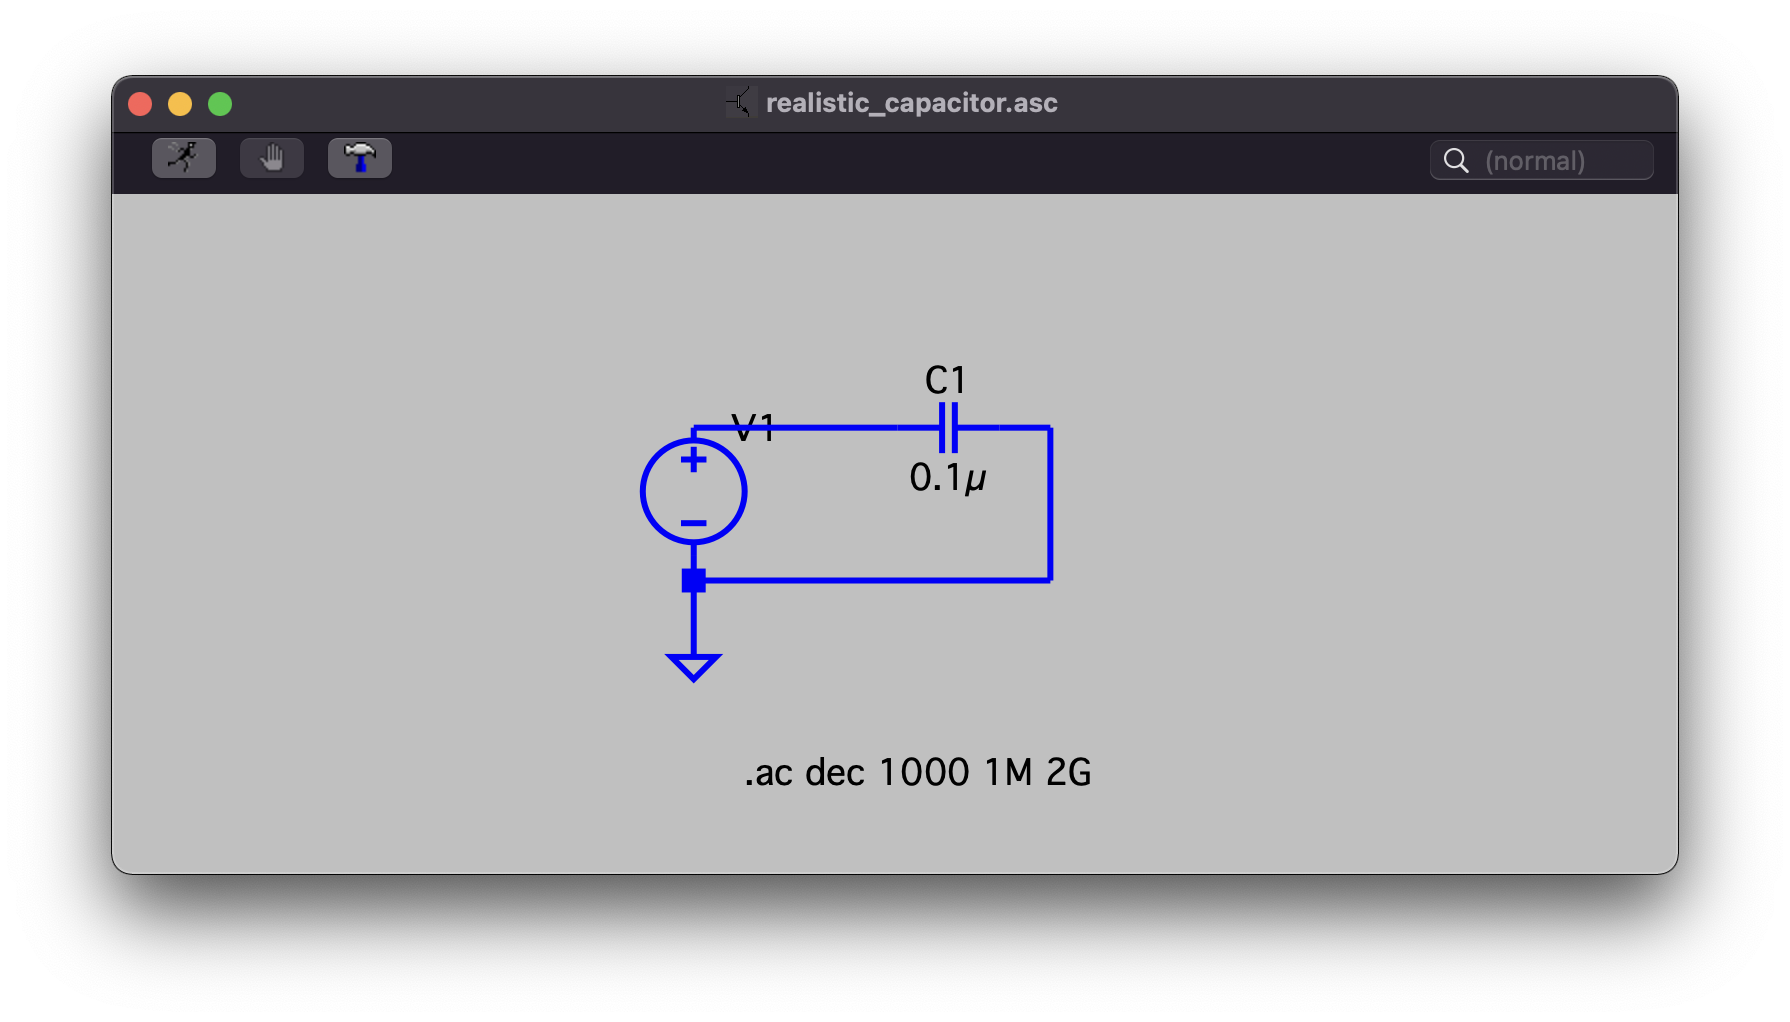
\includegraphics[width=\textwidth]{images/realistic_capacitor_setup.png}
\end{figure}
The circuit looks innocent, but  as often is the case in reality, the devil is in the details; here we show the parasitics modeled by the capacitor.
\begin{figure}[H]
    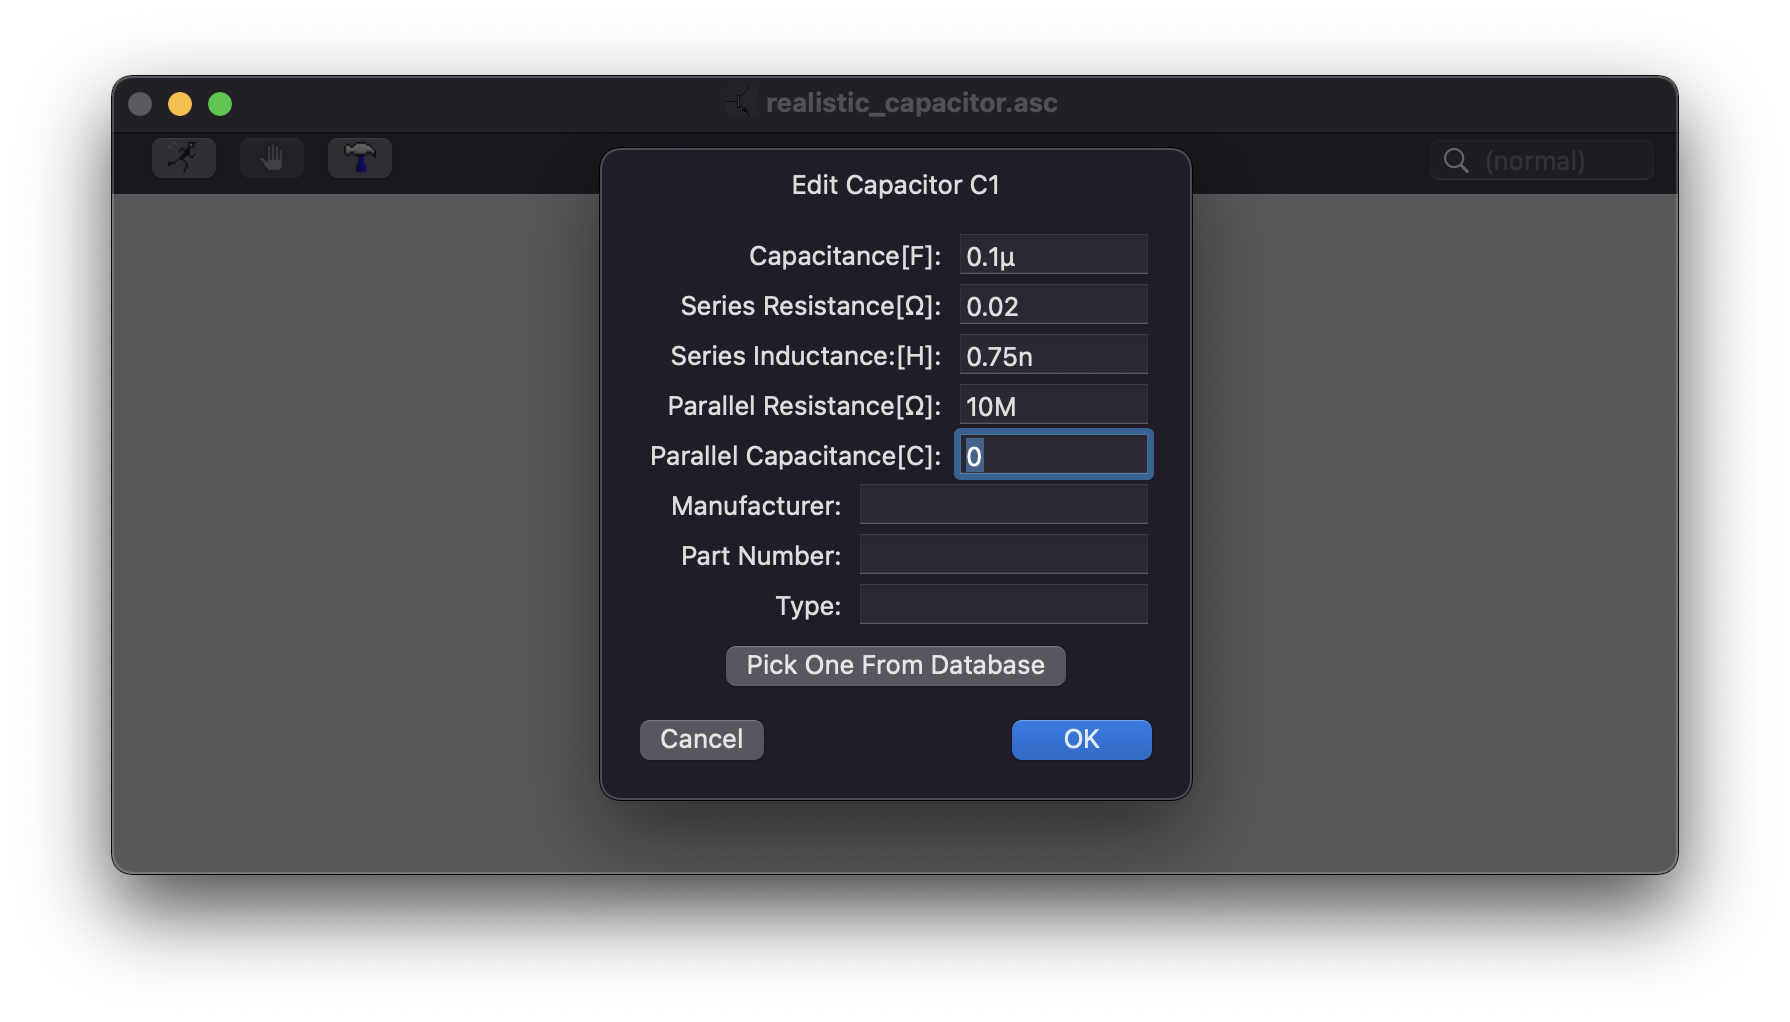
\includegraphics[width=\textwidth]{images/realistic_capacitor_setup_parasitics.png}
\end{figure}
Through an AC analysis we can observe the actual impedance of the capacitor.
\begin{figure}[H]
    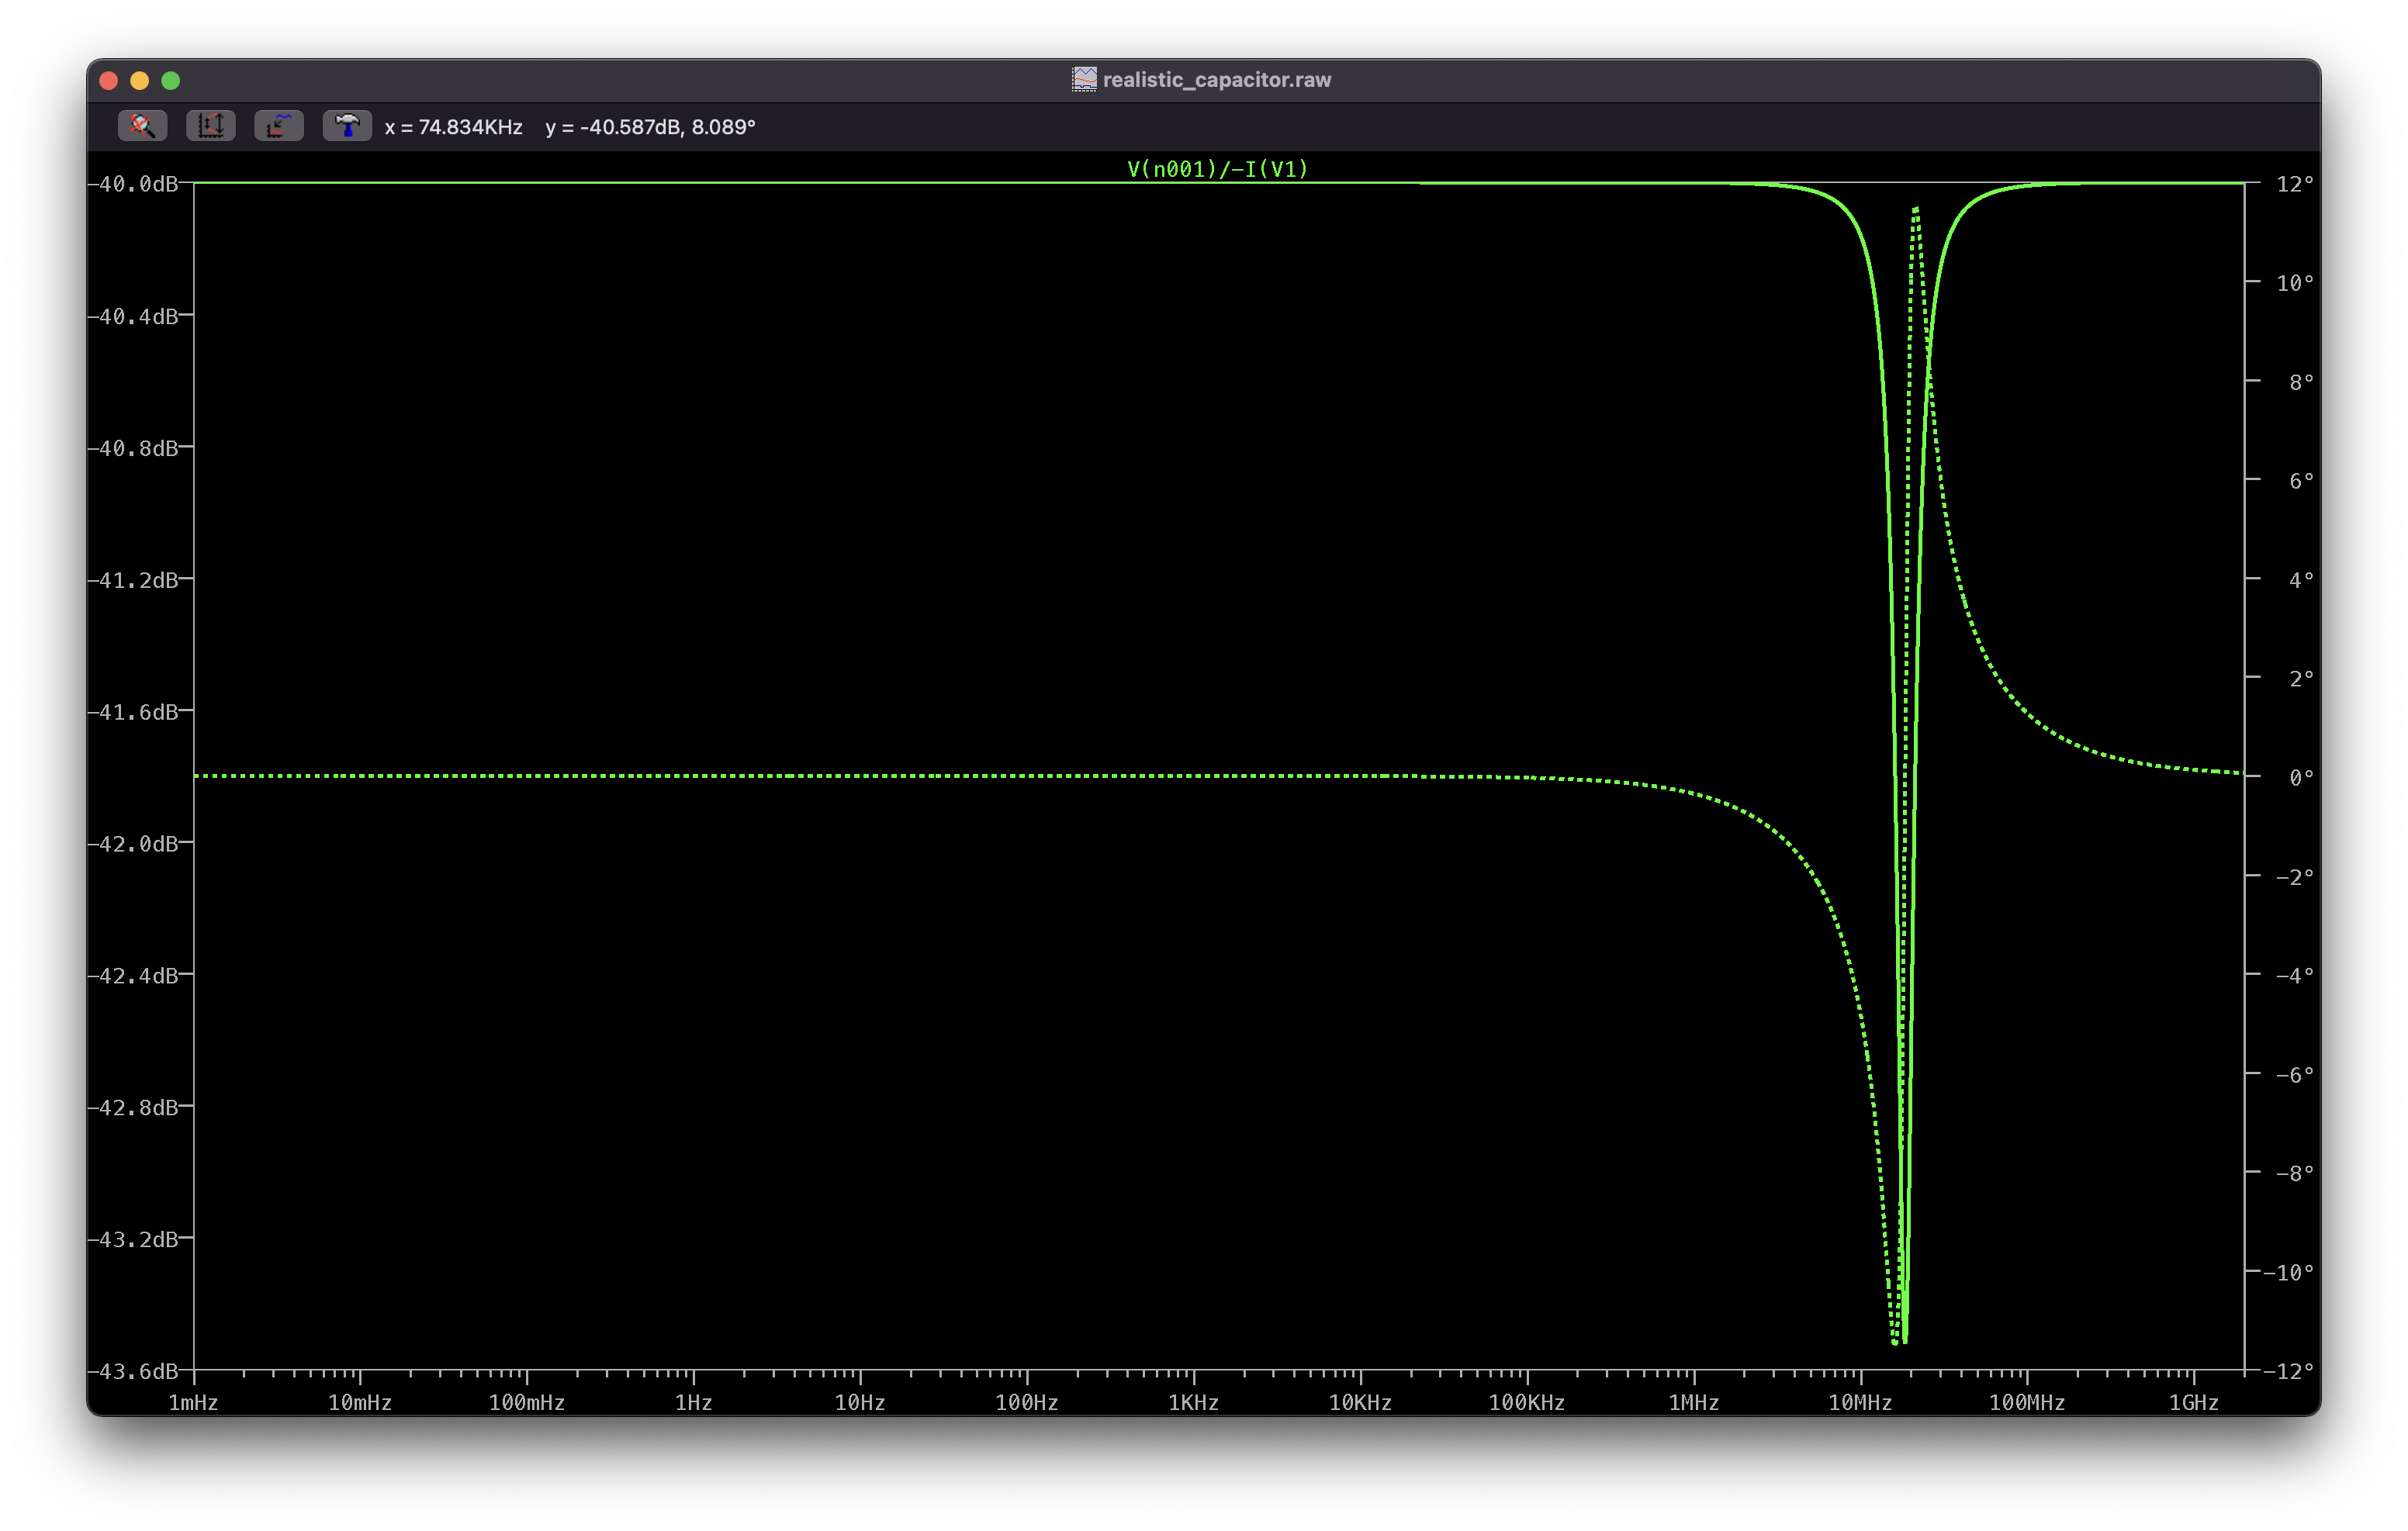
\includegraphics[width=\textwidth]{images/ltspice_realistic_capacitor.png}
    \caption{Realistic Impedance of a Capacitor.}
\end{figure}
Note the capacitor has a resonant frequency around 19 MHz. From our theoretical understanding of a capacitor's impedance, we'd expet $Z_{C} = 1/{j\omega C}$, where $\omega = 2\pi f$ and $f$ being frequency - an inverse relationship.
For a realistic capacitor we clearly observe a difference impedance versus frequency relationship.
The location of the resonant frequency is a function of the vlaues of the capacitor and its various parasitics. An investigation into this relationship is left to the reader as an exercise.

\pagebreak

\section*{LTSpice Model of a Realistic Indudctor}
The reactant dual of the capacitor is the inductor. The testbench used to study its nonidealities is shown below.
\begin{figure}[H]
    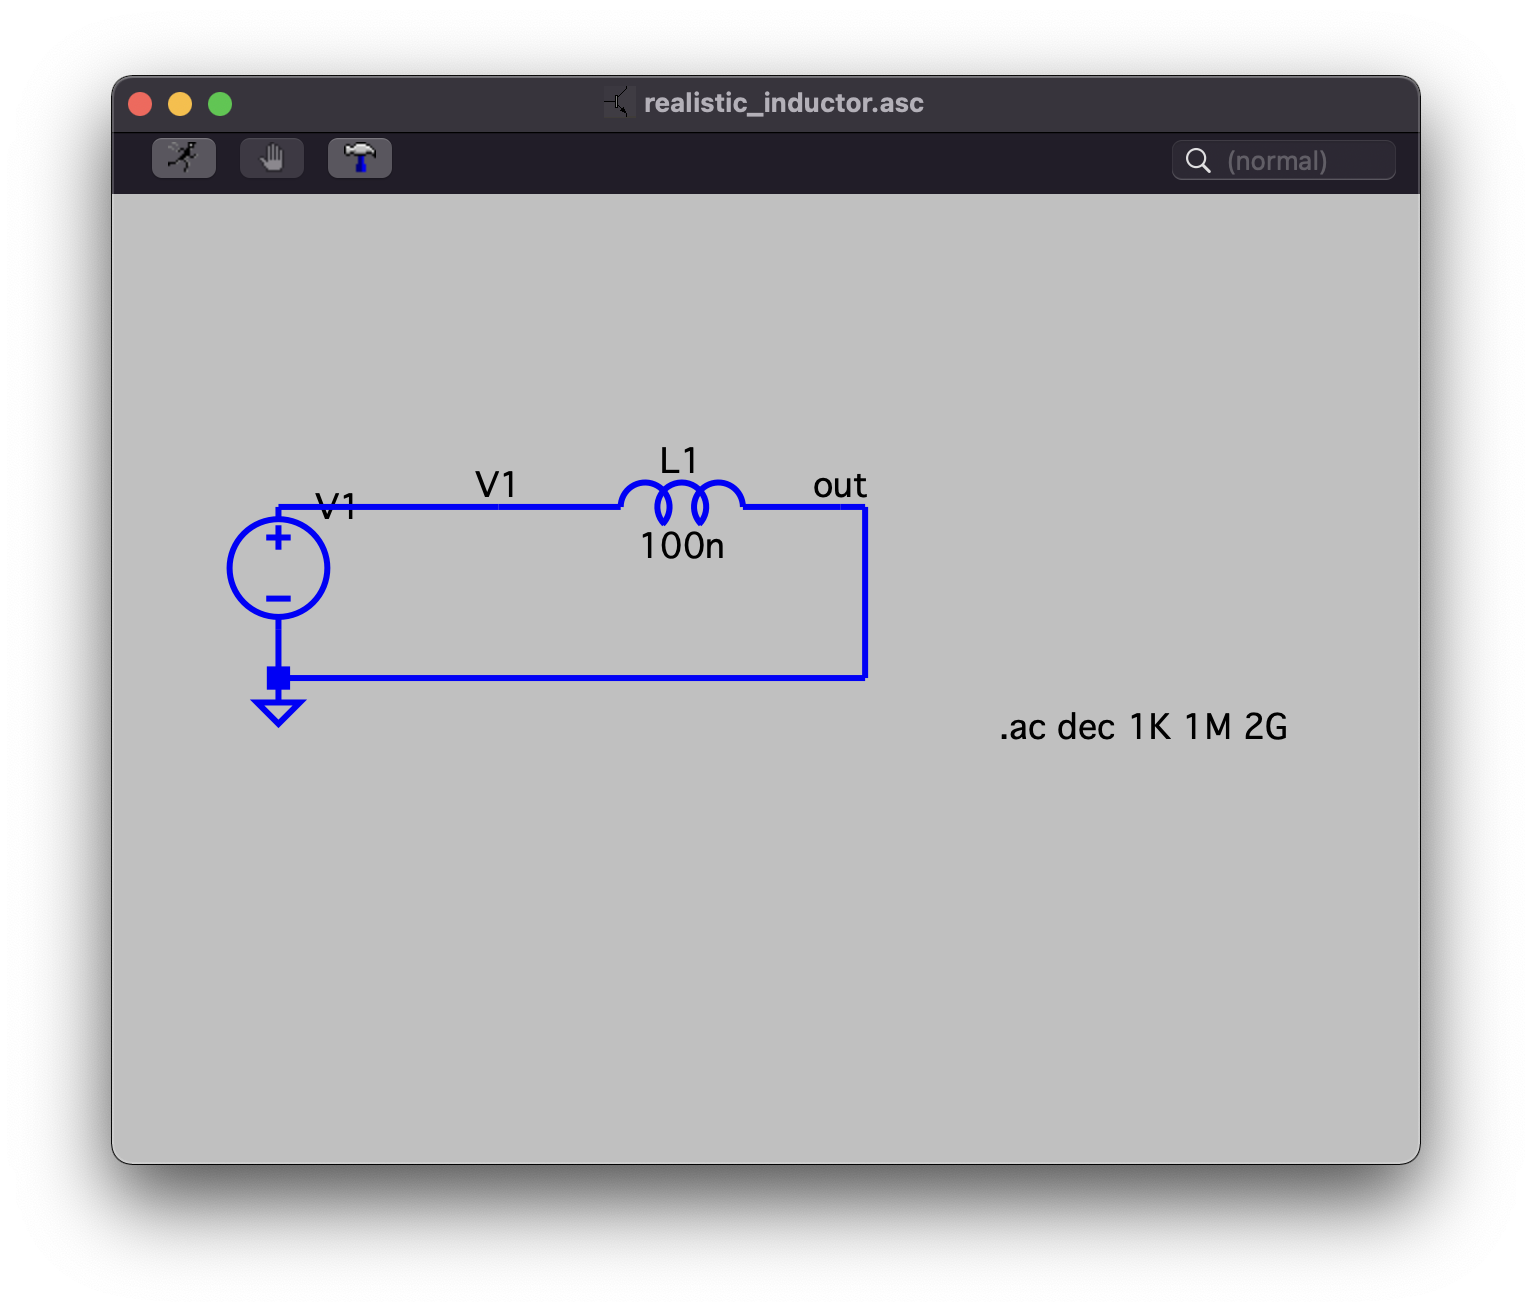
\includegraphics[width=\textwidth]{images/realistic_inductor_setup.png}
\end{figure}
The nonidealities in this example are as follows:
\begin{figure}[H]
    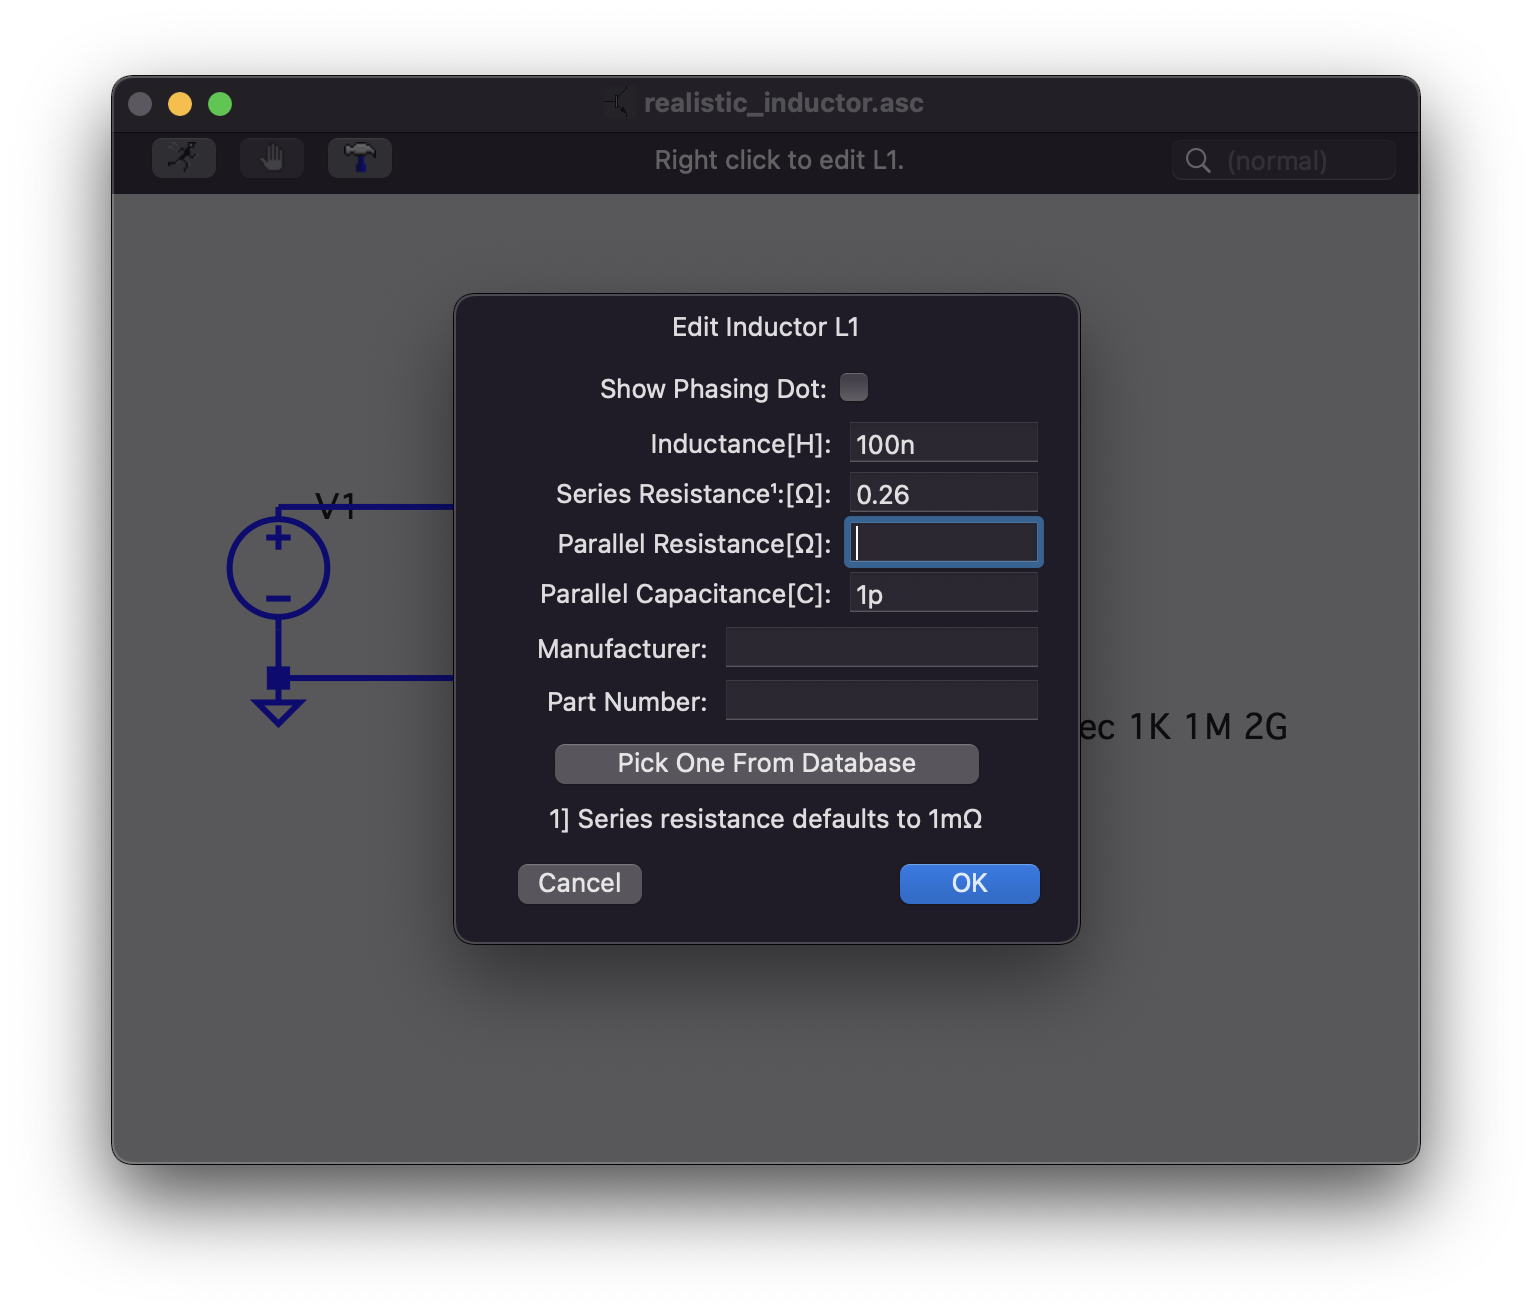
\includegraphics[width=\textwidth]{images/realistic_inductor_setup_parasitics.png}
\end{figure}
The reason for excluding the parallel resistance $R_p$ is that in this case we assume $R_p$ is very large. Note that if $R_p$ were small, then $R_p$ would provide an alternate path for current to flow at all frequencies.
The impedance versus frequency for the realistic inductor model is shown below:
\begin{figure}[H]
    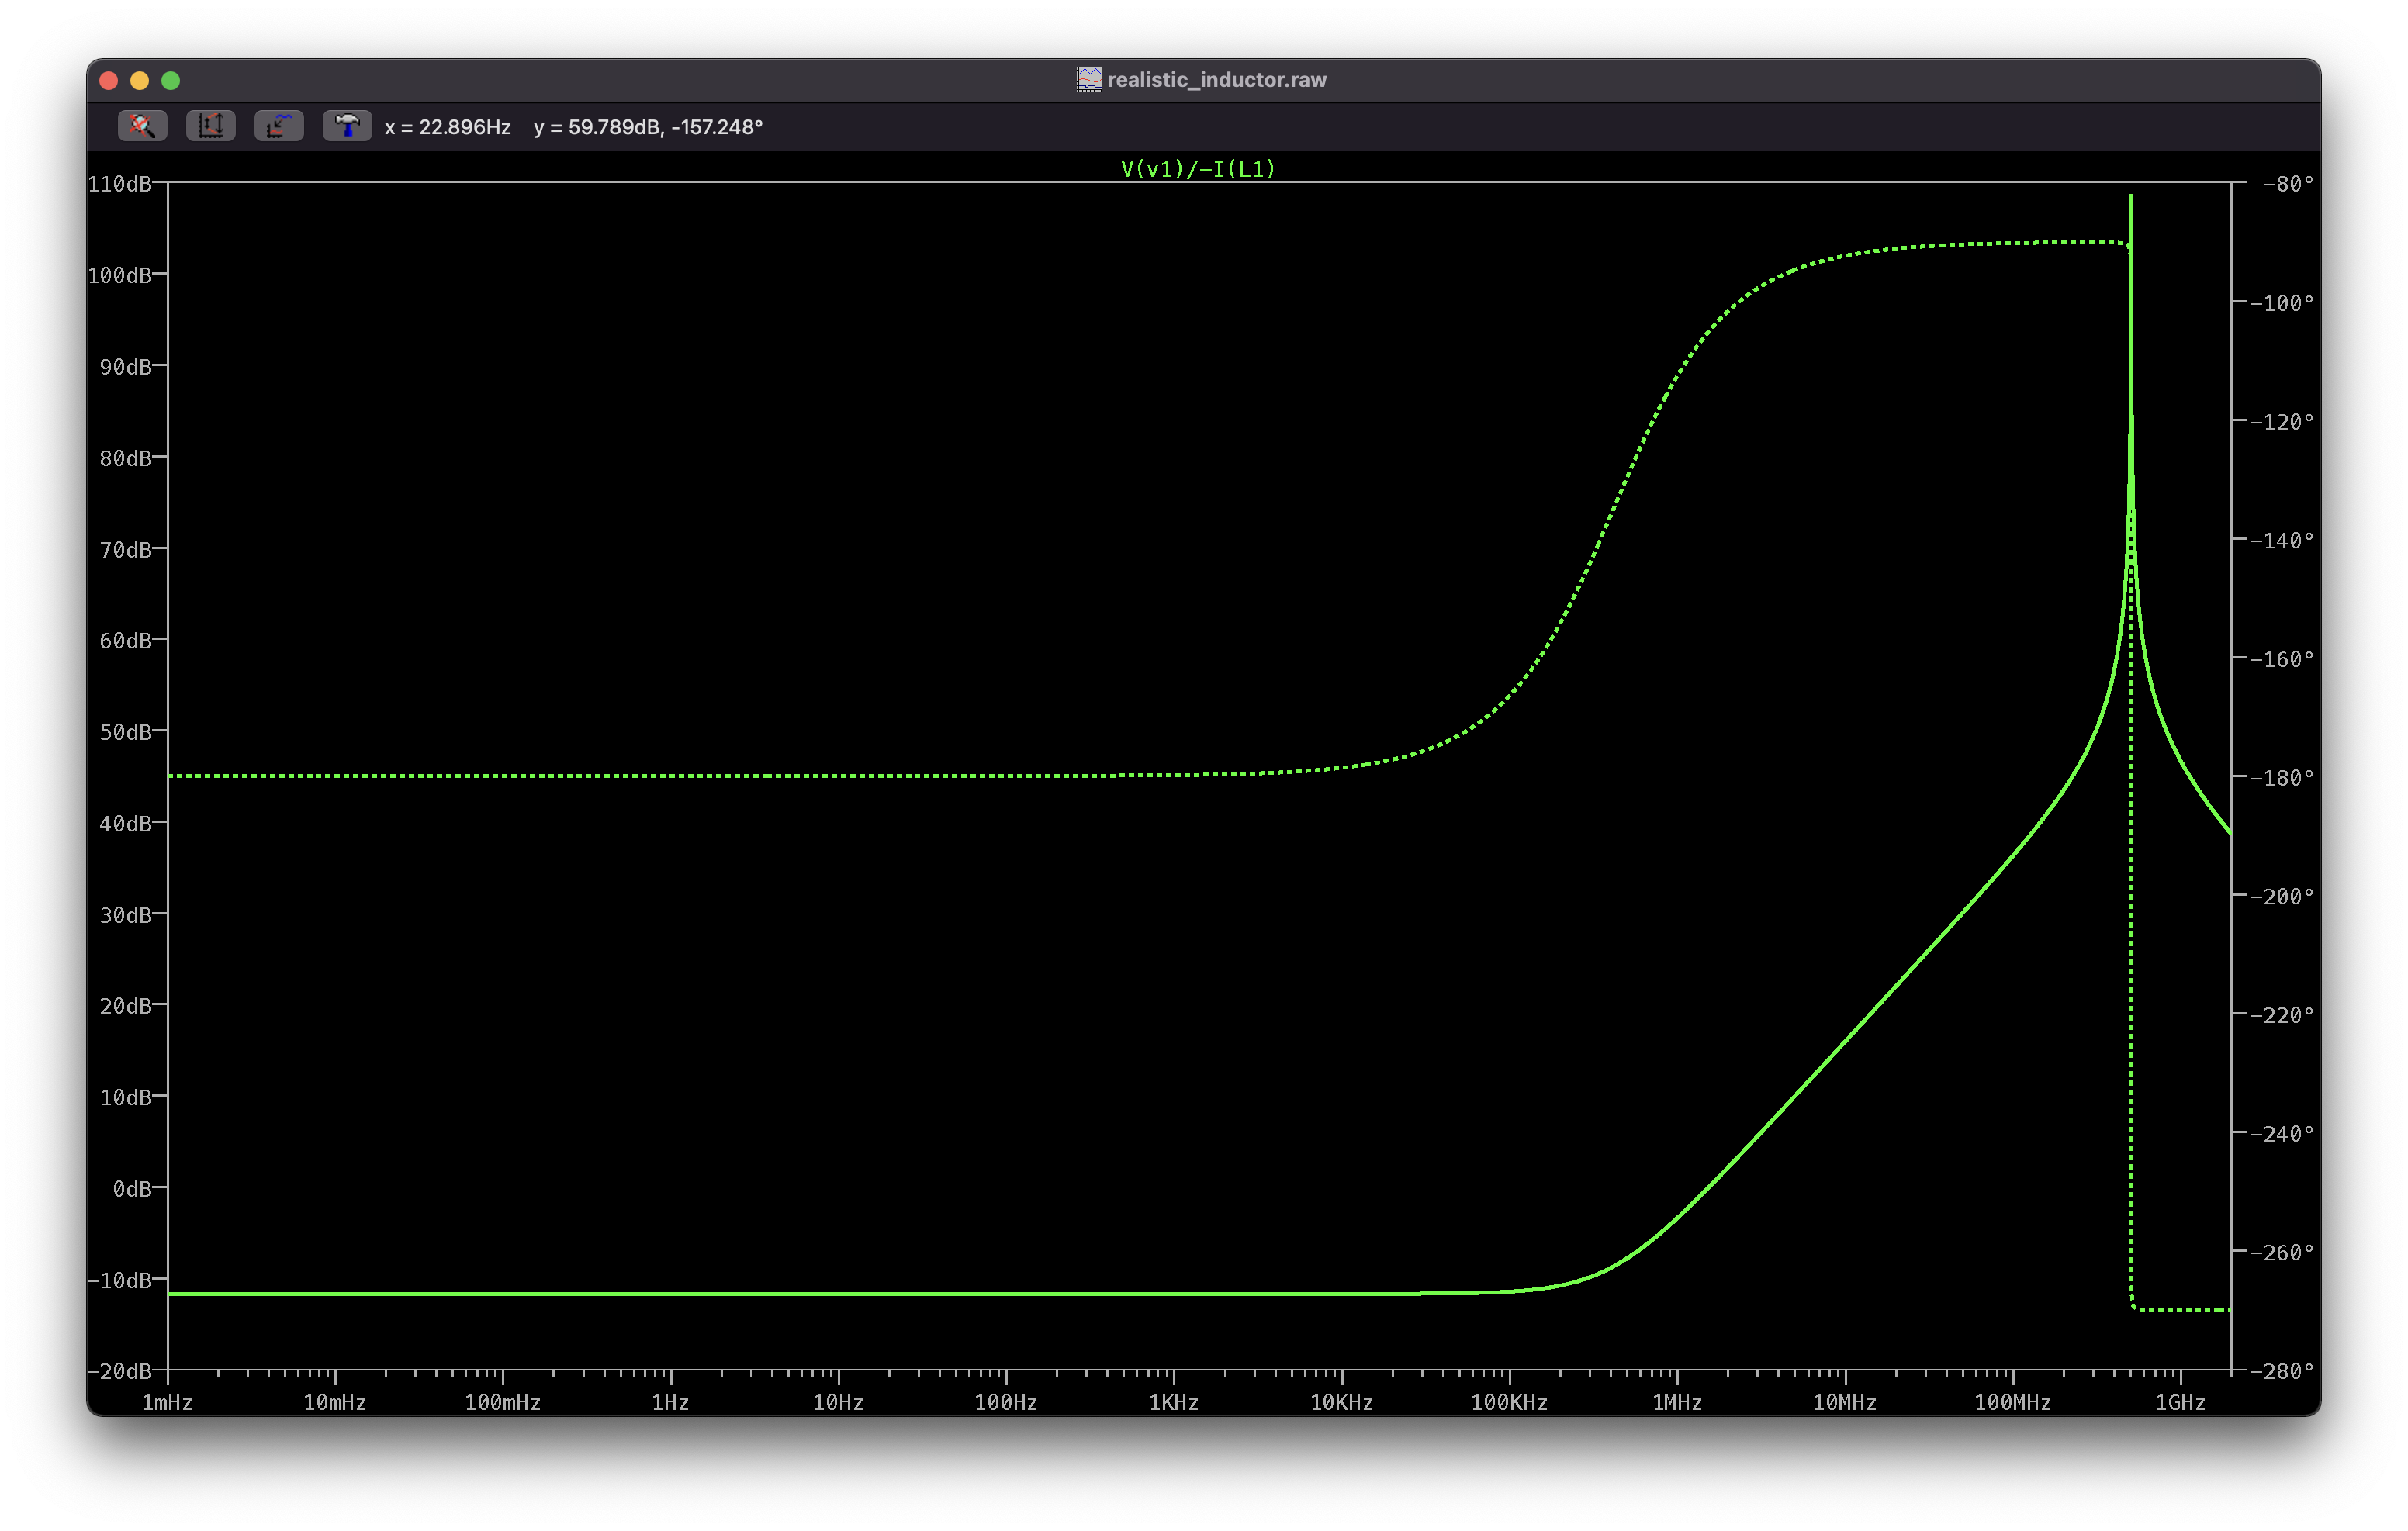
\includegraphics[width=\textwidth]{images/ltspice_realistic_inductor.png}
\end{figure}

From our textbook circuit knowledge we know inductors have an idela impedance of $L_c = j\omega L$.
Note that like the capacitor, the inductor too has a reasonant frequency. In the inductor's case, the resonant frequency is around 500 MHz. 
\\\\
An interesting duality between these two reactive components is the direction the peaking. For high Q (Q is the quality factor, and can be defined as the magnitude of the impedance at its resonant frequency), the inductor's impedance increases dramatically. The capacitor's impedance decreases significantly.
The mathematical intuition behind this is that the reactant components have opposite signs in their model of impedance. Recall $Z_c = 1/j\omega C$. Note that $Z_c = 1/j\omega C = -j/\omega C$.

\pagebreak

\section*{Lab Measurements}
\subsection*{Capacitor}
\subsection*{Inductor}
\end{document}